\documentclass{lab}

\begin{document}
	
\labtitle{1.4.8}{Электромагнитные волны в волноводах}{3 ноября 2018 г.}{10 ноября 2018 г.}

\section*{Постановка эксперимента}
\begin{quote}
	\textbf{{\normalsize Цель работы: }}
	ознакомление с методами получения и анализа электромагнитных волн СВЧ-диапазона.
\end{quote}
\begin{quote}
	\textbf{{\normalsize Оборудование: }}
	генератор СВЧ типа Г4-83, измерительная линия Р1-28, усилитель 28 ИМ, заглушка, отрезок
	волновода с поглощающей нагрузкой, отрезки волноводов различных сечений, детекторная
	головка.
\end{quote}

\subsection*{Теоретическая часть}
\hspace{\parindent}
Передача энергии электромагнитных (э.м.) колебаний низкой частоты
(скажем, 50 Гц) не представляет проблем и делается широко известным
способом — по проводам. На более высоких частотах (до 300 МГц) эта
задача решается с помощью двухпроводных линий и коаксиальных кабелей.
На ещё более высоких частотах (до 300 ГГц), при колебаниях с
длинами волн (в вакууме) от 1 метра до 1 миллиметра (этот диапазон
называется диапазоном сверхвысоких частот или, сокращённо, СВЧ),
передача энергии с помощью двухпроводной линии или коаксиальных
кабелей становится малоэффективной из-за больших потерь: во-первых,
резко возрастает сопротивление проводов из-за скин-эффекта — вытеснения
тока на поверхность, а в двухпроводной линии, кроме
того, потери растут вследствие излучения энергии в окружающее пространство $(\sim \nu^4)$.

В СВЧ-диапазоне энергия передаётся с помощью металлических труб,
называемых волноводами. Электромагнитные волны
могут распространяться по металлическим трубам любого профиля,
но из технологических соображений сечения волноводов делаются либо
круглыми, либо прямоугольными.

В волноводе прямоугольного сечения может распространяться э.м. волна,
которую в пределах волновода можно рассматривать как результат суперпозиции двух плоских волн.
Каждая плоская волна является чисто поперечной, так что электрическое и магнитное поля
перпендикулярны к направлению их распространения. В суммарной волне электрическое поле имеет
только составляющую $E_y$ и, следовательно, перпендикулярно оси волновода,
а магнитное поле имеет составляющие $H_x$~и~$H_z$.

{\it Электромагнитное поле в волноводе не является чисто поперечным, а имеет продольные составляющие.}\\

В работе будем использовать обозначения: $k$ -- волновое число, $\lambda$ -- длина волны,
$\omega$ -- круговая частота, $v_ф$ -- фазовая скорость (в вакууме равна скорости света).
$$ k = \dfrac{2\pi}{\lambda} = \dfrac{\omega}{v_ф} $$
Для э.м. волны с начальной фазой $\varphi_0$ векторы напряженностей $\ve{E}$ и $\ve{H}$
удовлетворяют волновым уравнениям типа:
\begin{equation}
\begin{cases}
\nabla^2\ve{E} = \dfrac{1}{v^2}\dd{^2\ve{E}}{t^2}\\
\nabla^2\ve{H} = \dfrac{1}{v^2}\dd{^2\ve{H}}{t^2}
\end{cases}
\then
\begin{cases}
E=E_0\cos(\omega t - kx + \varphi_0)\\
H=H_0\cos(\omega t - kx + \varphi_0)
\end{cases}
\end{equation}

\begin{wrapfigure}[10]{l}{5cm}
	\vspace{-0.5cm}
	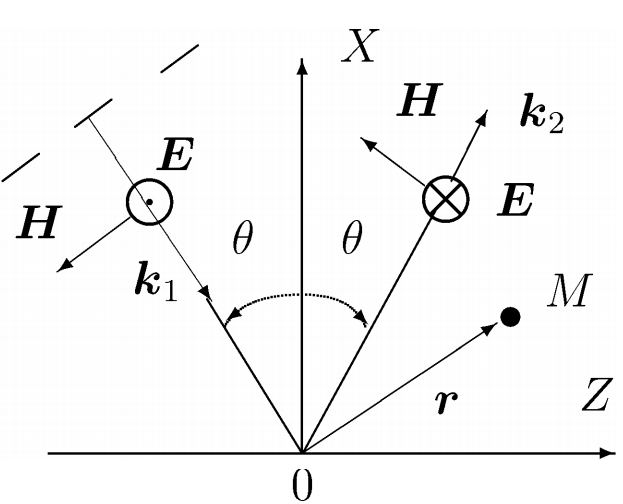
\includegraphics[width=5cm]{0}
	\caption{\footnotesize}
	\label{1}
\end{wrapfigure}

Рассмотрим отражение плоской э.м. волны от идеально проводящей,
бесконечно протяжённой плоской поверхности $x = 0$ (рис. \ref{1}). Пусть вектор
напряжённости электрического поля падающей волны $\ve{E}$ параллелен
этой плоскости. В наших обозначениях вектор $ve{E}_{пад}$ направлен по оси $Y$
(на нас). Фронт волны, падающей под углом $\Theta$ к нормали, показан на
рис. \ref{1} пунктиром. Оба вектора напряжённости $\ve{E}~и~\ve{H}$ лежат в плоскости
фронта волны, им перпендикулярен волновой вектор $\ve{k}$, описывающий
распространение волны.

Суммарное электрическое поле в произвольной точке M(x,0,z) имеет вид:
$$ E = 2iE_0\sin(kx\cos\Theta)e^{i\omega(t-z\sin\Theta/c)} $$
Это выражение для волны с амплитудой $2iE_0\sin(kx\cos\Theta)$, бегущей по направлению $z$
с фазовой скоростью $v_Ф = {c}/{\sin\Theta}$

При фиксированном угле $\Theta$ амплитуда поля гармонически зависит от $x$ и не меняется со
временем. Иначе говоря, в результате интерференции падающей и отражённой волн в пространстве
над проводящей поверхностью в направлении оси $X$ образуется система
стоячих волн. Электрическое поле стоячей волны равно нулю в точках,
где $kx \cos \Theta = n\pi$, т.е. там, где:
$$ x = \dfrac{n\pi}{k\cos\Theta};~~~~~~~n = 0, 1, 2, \dots$$

Если даны две параллельные проводящие плоскости, расположенные на расстоянии $a$ друг от друга,
то $\omega_{кр} = \pi c/a, ~ \lambda_{кр} = 2a$

Фазовая скорость (скорость перемещения поверхности постоянной фазы $v_ф~=~\omega/k$) в волноводе больше скорости света в пустоте, а групповая (скорость распространения возмущения 
$u = d\omega/dk$) всегда меньше. Интересно отметить, что фазовая скорость зависит от частоты.

Если в волноводе имеется какое-либо препятствие, нерегулярность (в предельном случае он просто
закрыт металлической пластиной), то в нём появляется отражённая волна. Падающая
и отражённая волны интерферируют и создают в волноводе стоячую волну, похожую на стоячие
волны в струне. Запишем прямую волну, движущуюся в положительном
направлении оси $Z$, и отраженную в виде:
$$ E_1 = E_0 e^{i(\omega t - k_zz)} ~~~~~ E_2 = E_0 \rho e^{i(\omega t + k_zz + \varphi)} $$
где $\rho$ -- коэффициент отражения по амплитуде, а $\varphi$ -- фаза отраженной волны.
Суммарное поле в волноводе имеет вид:
$$ E(z) = E_1 + E_2 = E_0e^{-ik_zz}(1+\rho e^{i(2k_zz+\varphi)})e^{i\omega t} = A_0e^{i\omega t} $$
Максимальное (в пучности) и минимальное (в узле) значения поля равны соответственно:
$$ E_{max} = E_0(1+\rho)~~~~~~~E_{min} = E_0(1-\rho) $$
Расстояние между двумя узлами $l = \pi/k_z = \lambda_в/2$. Отношение $K = E_{max}/E_{min}$
называется {\it коэффициентом стоячей волны} (к.с.в.).
$$ \rho = \dfrac{E_{max} - E_{min}}{E_{max} + E_{min}} = \dfrac{K - 1}{K + 1} $$

\subsection*{А. Волны в волноводе при частоте выше критической}
\subsubsection*{Экспериментальная установка}

Схема для исследования структуры волн в волноводе при частоте выше критической представлена
на рис. \ref{ust1}. Модулированный сигнал от высокочастотного генератора поступает на вход
A измерительной линии, вдоль которой перемешается зонд~S. Высокочастотный сигнал с зонда поступает
на кристаллический детектор D.

\begin{figure}[H]
	\centering
	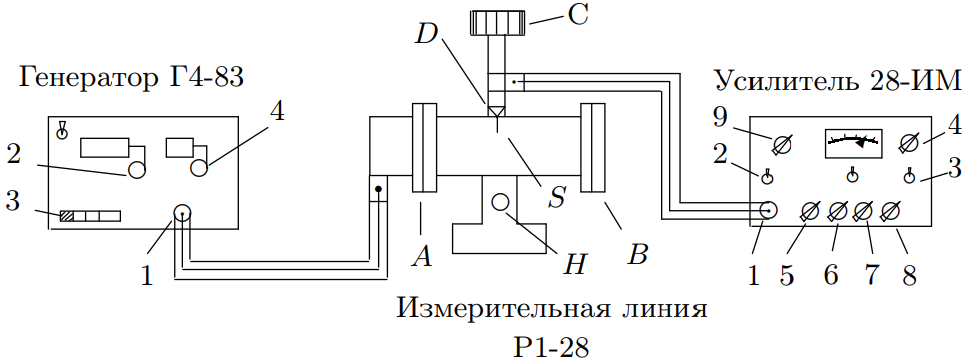
\includegraphics[width = 0.7 \textwidth]{ust1}
	\caption{\footnotesize
		Схема для исследования структуры волн СВЧ
	}
	\label{ust1}
\end{figure}

Определив расстояние между узлами, можно рассчитать длину волны и фазовую скорость СВЧ-сигнала в
волноводе. Устройство детекторной головки, установленной на измерительной линии,
таково, что отклик вольтметра U на величину напряжённости электрического поля E в волноводе.
$$ U \sim E^n $$
По графику по графику $\ln(U) = f[\ln(E)]$ можно определить $n$, если известно распределение
поля $E(z)$. Распределение $E(z)$ нетрудно рассчитать для волновода с закороченным
концом (металлической заглушкой), когда фаза отражённой волны $\varphi = \pi,~а~\rho = 1$. При этом:
$$ E(z) = E_0e^{-ik_zz}(1 - e^{2ik_zz})e^{i\omega t} = E_0e^{i\omega t}(e^{-ik_zz}-e^{ik_zz})
= 2E_0e^{i\omega t}\sin(k_zz) \sim \sin(k_zz) $$

Меняя нагрузку на выходе измерительной линии (B на рис. \ref{ust1})
и сравнивая максимальное и минимальное показания вольтметра, можно
рассчитать коэффициент стоячей волны (к.с.в.) и коэффициент отражения $\rho$.

\subsection*{Б. Волны в волноводе при частоте ниже критической}

\begin{figure}[H]
	\centering
	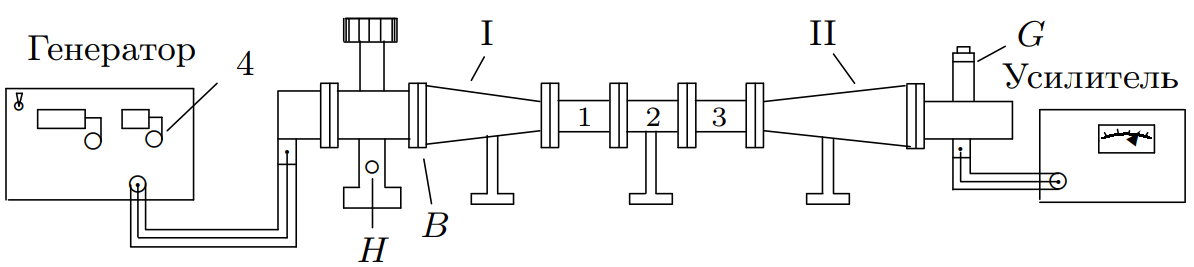
\includegraphics[width = 0.7 \textwidth]{ust2}
	\caption{\footnotesize
		Схема для исследования затухания
	}
	\label{ust2}
\end{figure}

Для исследования затухания волн в волноводе при частоте ниже критической используются те
же генератор, усилитель, измерительная линия и дополнительный набор волноводов с отдельной детекторной головкой
G (рис. \ref{ust2}). Дополнительный набор начинается и заканчивается волноводами
переменного сечения I и II. Между ними можно разместить 1, 2 или 3 одинаковых отрезка с постоянным сечением.
В такой системе волны с частотами меньше критической экспоненциально затухают.
Мощность сигнала на выходе из волновода $W$ можно связать с мощностью входного сигнала
$W_0$ двумя способами:
\begin{equation}
\begin{aligned}
&W = W_0e^{-\alpha z} ~или~ W = W_010^{-\beta z} ~~~~~ z - длина ~ волновода.\\
&(\beta z) = 10 \lg \dfrac{W_0}{W} ~~~~~~~ \alpha = 2.3 \cdot \beta\\
&\alpha = 2ik = \dfrac{2\omega}{c}\sqrt{\left(\dfrac{\omega_{кр}}{\omega}\right)^2 - 1} = 
\dfrac{2\pi}{a}\sqrt{1 - \left(\dfrac{2a}{\lambda_0}\right)^2}
\end{aligned}
\end{equation}

\section*{Выполнение эксперимента}
В работе предлагается при частоте выше критической исследовать
стоячую волну в измерительной линии (рис. \ref{ust1}): измерив распределение
сигнала вдоль волновода, рассчитать фазовую скорость и определить характер
детектирования (линейный, квадратичный и т.д.); затем, меняя
нагрузку на выходе волновода (заглушка, открытый конец или поглотитель),
определить коэффициенты отражения электромагнитной волны. При частоте ниже критической предлагается определить
коэффициент затухания волны в сборном волноводе (рис. \ref{ust2}) и сравнить с теоретическим.
\subsection*{Измерения и вычисления}
\subsection*{А. Волны в волноводе при частоте выше критической}
\subsubsection*{Определение длины волны СВЧ-сигнала в волноводе}
\begin{enumerate}
\item Восстановим рабочую частоту $\nu = 9320~МГц$ и снимем зависимость показаний вольтметра
$U$ от положения зонда $z$. Установим также ослабление выходной мощности $\gamma = 20$ дБ.
При этом $\lambda_0 = {c}/{\nu_0}=32~мм,~\lambda_{кр} = 2\cdot a = 46~мм.$
\begin{table}[H]
	\centering
	\begin{tabular}{|c|ccccccccccccccccc|}
		\hline
		$z,~мм$		&0	&1	&2	&3	&4	&5	&6	&7	&8	&9	&10	&11	&12	&13	&14	&15	&16	\\ %\hline
		$U,~мкВ$	&36	&27	&19	&11	&5	&1	&0	&1	&5	&13	&22	&30	&40	&49	&58	&65	&69	\\ \hline \hline
		$z,~мм$		&17	&18	&19	&20	&21	&23	&24	&25	&26	&27	&28	&30	&31	&33	&35	&37	&40	\\ %\hline
		$U,~мкВ$	&71	&70	&67	&61	&52	&32	&22	&12	&5	&1	&0	&5	&11	&25	&42	&56	&65	\\ \hline
	\end{tabular}
	\caption{\footnotesize 
		Зависимость $ U=f(z) $
	}
	\label{tab1}
\end{table}

Вычислим длину волны $ \lambda_в $ в волноводе.

\begin{equation}
\lambda_в = \dfrac{\lambda_0\lambda_{кр}}{\lambda_{кр}^2 - \lambda_0^2} = \dfrac{32 \cdot 46}{46^2 - 32^2} = 44.5~мм
\end{equation}

\newpage

\item Построим график $U = f(z)$ используя данные из таблицы \ref{tab1}.

\begin{figure}[H]
	\centering
	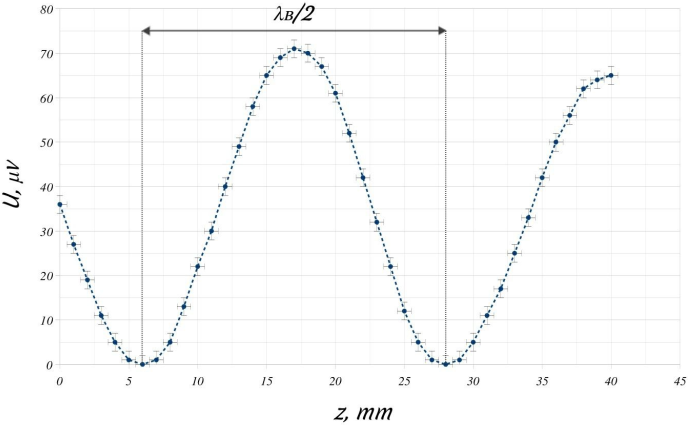
\includegraphics[width = 0.9 \textwidth]{1}
	\caption{\footnotesize
		График зависимости показаний вольтметра $ U $ от положения зонда $ z $.
	}
	\label{graph1}
\end{figure}

Из графика \ref{graph1} находим значение $ \lambda_в = 44~мм. $

Рассчитаем также фазовую скорость $ v_ф $ волн в волноводе, групповую скорость $ u $, используя
соотношение $ v \cdot v_ф = c^2 $, и волновое число $ k $, описывающее распространение волны вдоль волновода.

\begin{equation}
\begin{aligned}
&v_ф = \nu_0 \cdot \lambda_в = 4.1 \cdot 10^8~м/с\\
&u = \dfrac{c^2}{v_ф} = 2.2 \cdot 10^8~м/с\\
&k = \dfrac{\omega_0}{v_ф} = \dfrac{2\pi\nu_0}{v_ф}
\end{aligned}
\end{equation}

\subsubsection*{Определение характера детектирования}

\item Установим зонд в узел стоячей волны ($ U=U_{min} $). Снимем зависимость $ U $ от
координаты зонда $ x $ внутри выбранного диапазона.

\begin{table}[H]
	\centering
	\begin{tabular}{|c|ccccccccccccccc|}
		\hline
		$x,~мм$		&2.9&3.0&3.2&3.6&4.2&4.7&5.2&5.9&6.6&7.2&7.5&8.2&8.4&8.7&8.8\\ %\hline
		$U,~мкВ$	&12&11&10&8&6&5&3&0&3&5&6&8&10&11&12\\ \hline \hline
		$\ln(kz)$	&1.4&1.4&1.4&1.2&1.0&0.9&0.6&-&0.6&0.9&1.1&1.2&1.3&1.4&1.4 \\
		$\ln(U)$	&2.5&2.4&2.3&2.1&1.8&1.5&0.9&-&0.9&1.5&1.8&2.1&2.3&2.4&2.5 \\ \hline
	\end{tabular}
	\caption{\footnotesize 
		Зависимость $ U $ от координаты зонда $ x $, где $ z=\abs{x-x_0} $,\\
		а $ x_0 $ -- координата узла стоячей волны.
	}
	\label{tab2}
\end{table}

\item Построим график $ \ln(U) = f\{\ln\left[\sin(kz)\right]\} $.

\begin{figure}[H]
	\centering
	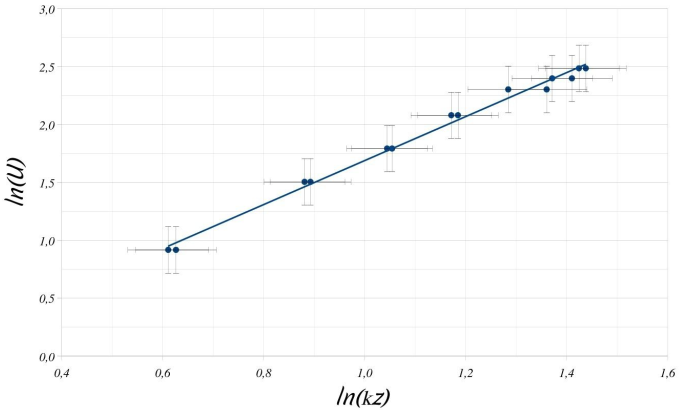
\includegraphics[width = 0.9 \textwidth]{2}
	\caption{\footnotesize
		График зависимости показаний вольтметра $ U $ от сдвига узла на $ z $.
	}
	\label{graph2}
\end{figure}

Из графика \ref{graph2} по наклону прямой определим характер детектирования $ U \sim E^n $:
$ n \simeq 2 $. Следовательно, у нас квадратичный характер детектирования.

\subsubsection*{Определение коэффициентов отражения}

\item Снимем металлическую заглушку с фланца измерительной линии. Перемещая зонд определим
максимальное и минимальное напряжения в волне. Затем наденем поглощающую нагрузку, снова
измерим максимальное и минимальное напряжения в волне. Определим коэффициент отражения
$ \rho $ для открытого и закрытого волноводов и для волновода с поглощающей нагрузкой.

$$ \rho = \dfrac{K-1}{K+1},~~~~~ где ~ K = \dfrac{E_{max}}{E_{min}} =
\left( \dfrac{U_{max}}{U_{min}} \right)^{1/2} $$

\begin{table}[H]
	\centering
	\begin{tabular}{|c|cc|}
		\hline
					&\hspace*{0.5cm} $ \rho $ \hspace*{0.5cm}	&\hspace*{0.5cm} $ K $ \hspace*{0.5cm}		\\ \hline
		Без нагрузки&0.34		&2			\\
		С нагрузкой	&0.1		&1.1		\\
		Зеркало		&1			&$\infty$	\\ \hline
	\end{tabular}
\caption{\footnotesize
	Коэффициенты отражения при разных выходах на волноводе.
}
	\label{tabrho}
\end{table}

\subsection*{Б. Волны в волноводе при частоте ниже критической}
\subsubsection*{Измерение коэффициент затухания}

\item Соберем установку по схеме, изображенной на рисунке \ref{ust2}. Для добавочных
отрезков волноводов $ a = 16 $ мм. Следовательно, $ \lambda_{кр} = 32~мм $. При этом
$ \lambda_0~=~46~мм $. Это значит, что $ \nu_0 = 9320~МГц < \nu_{кр} = 9375~МГц $.

\item Установим минимальное затухание $ \gamma = 20~дБ $. Последовательно уменьшая
число промежуточных секций,каждый раз подберем ослабление $ \gamma $ сигнала, при
котором показания вольтметра усилителя остаются неизменными.

\begin{table}[H]
	\centering
	\begin{tabular}{|c|ccccccc|}
		\hline
		$ z,~см $		&43.9	&39.9	&38.8	&38.0	&34.9	&34.1	&33.2	\\
		$ \gamma,~дБ $	&20.0	&25.3	&27.7	&28.4	&34.4	&35.9	&37.7	\\ \hline
	\end{tabular}
	\caption{\footnotesize 
		Зависимость минимального затухания $ \gamma $ от длины всего волновода $ z $.
	}
	\label{tab3}
\end{table}

\item Построим график в удобных координатах по данным таблицы \ref{tab3}.

\begin{figure}[H]
	\centering
	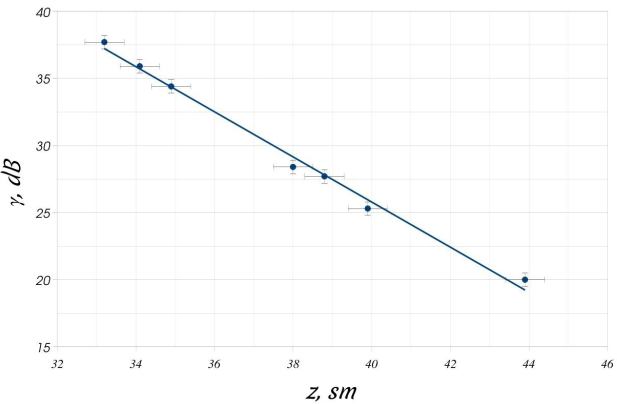
\includegraphics[width = 0.9 \textwidth]{3}
	\caption{\footnotesize
		График зависимости минимального затухания $ \gamma $ от длины всего волновода $ z $.
	}
	\label{graph3}
\end{figure}

Из графика \ref{graph3} определяем:

\begin{equation}
\begin{aligned}
&\beta = 0.168~Б/см\\
&\alpha = 0.38~Нп/см
\end{aligned}
\end{equation}

При этом теоретическое значение $ \alpha $:
$$ \alpha = \dfrac{2\pi}{a}\sqrt{1-\left(\dfrac{2a}{\lambda_0}\right)^2} = 0.39~Нп/см $$

\end{enumerate}

\newpage

\subsection*{Расчет погрешностей}
\subsubsection*{Источники погрешностей}

При измерениях длины детектора: $ \sigma_z = \sigma_x = 0.2~мм $.\\
На генераторе для затухания: $ \sigma_{\gamma} = 0.5~дБ $.\\
На вольтметре: $ \sigma_U = 1~мкВ $.\\
При измерении длины волновода линейкой: $ \sigma_l = 0.2~см $.

\subsubsection*{Систематическая погрешность}
\hspace*{\parindent}
При определении длины волны СВЧ-сигнала в волноводе:\\
$ \sigma_{\lambda_в} \simeq 2~мм $.\\
$ \sigma_{v_ф} = 2 \cdot 10^7~м/с $.\\
$ \sigma_u = 10^7~м/с $.\\
$ \sigma_k = 6 $.

При определении характера детектирования:\\
$ \sigma_{\ln(U)} = (1/u)\sigma_U $.\\
$ \sigma_z = \sqrt{2}\sigma_x, ~~~ где ~ z = \abs{x-x_0} $\\
$ \sigma_{\ln(kz)} = \left( \left(\dfrac{\sigma_k}{k}\right)^2 + \dfrac{2\sigma_x^2}{z^2} \right)^{1/2} $

При исследовании затухания волн:\\
$ \sigma_z = \sqrt{5}\sigma_l \simeq 0.5~см $

\subsubsection*{Случайная погрешность}

Для графика \ref{graph2} из МНК:
$ ~~~~~ \sigma_n \simeq 0.2 ~~~~~~ \varepsilon_n \simeq 13\% $\\
Для графика \ref{graph3} из МНК:
$ ~~~~~ \sigma_{\beta} \simeq 0.07 ~~~~~ \varepsilon_{\beta} = 4 \% $

\subsubsection*{Итоговые погрешности}

$ \sigma_n \simeq 0.3 \then \varepsilon_n \simeq 17 \% $\\
$ \sigma_{\beta} \simeq 0.07~дБ/см \then \varepsilon_{\beta} \simeq 4 \%$\\
$ \sigma_{\alpha} \simeq 0.02~Нп/см \then \varepsilon_{\alpha} = \varepsilon_{\beta}$

\section*{Итоги}

Определили длину волны СВЧ сигнала в волноводе теоретически и экспериментально, а также некоторое параметры для этой волны (записано выше):\\
$ \lambda_т = 44.5~мм, ~~~ \lambda_э = (44 \pm 2)~мм $\\
Установили характер детектирования в оборудовании, считывающей сигнал:\\ $ n = (1.9 \pm 0.3)
\then квадратичный ~ характер ~ (n = 2) $.\\
Также нашли коэффициенты отражения для разных случаев (см. таблицу \ref{tabrho}).\\
Определены коэффициенты мощностей для разных представлений:\\
\begin{equation}
W = W_0e^{-\alpha z} ~или~ W = W_010^{-\beta z} ~~~~~ z - длина ~ волновода.
\end{equation}
$$ \alpha_{теор} \simeq 0.39 ~ Нп/см $$
\begin{equation}
\begin{aligned}
&\beta = (0.168 \pm 0.007) ~ дБ/см &\then \varepsilon_{\beta} \simeq 4 \% \\
&\alpha = (0.38 \pm 0.02) ~ Нп/см  &\then \varepsilon_{\alpha} \simeq 4 \%
\end{aligned}
\end{equation}

\end{document}